% This LaTeX was auto-generated from MATLAB code.
% To make changes, update the MATLAB code and export to LaTeX again.

\documentclass{article}

\usepackage[utf8]{inputenc}
\usepackage[T1]{fontenc}
\usepackage{lmodern}
\usepackage{graphicx}
\usepackage{color}
\usepackage{hyperref}
\usepackage{amsmath}
\usepackage{amsfonts}
\usepackage{epstopdf}
\usepackage[table]{xcolor}
\usepackage{matlab}

\sloppy
\epstopdfsetup{outdir=./}
\graphicspath{ {./ayu1_images/} }

\begin{document}

\matlabheading{Ayudantía N°1}

\begin{par}
\begin{flushleft}
Estudiante: Valentina Andrade 
\end{flushleft}
\end{par}

\begin{par}
\begin{flushleft}
Magíster Economía PUC
\end{flushleft}
\end{par}

\matlabheading{Parte 1. Vectores y matrices}

\begin{par}
\begin{flushleft}
1. Genere tres variables escalares
\end{flushleft}
\end{par}

\begin{matlabcode}
a = 1
\end{matlabcode}
\begin{matlaboutput}
a = 1
\end{matlaboutput}
\begin{matlabcode}
b = 8
\end{matlabcode}
\begin{matlaboutput}
b = 8
\end{matlaboutput}
\begin{matlabcode}
c = 10
\end{matlabcode}
\begin{matlaboutput}
c = 10
\end{matlaboutput}

\begin{par}
\begin{flushleft}
2. Genere un vector columna
\end{flushleft}
\end{par}

\begin{matlabcode}
v1 = [a,b,c]
\end{matlabcode}
\begin{matlaboutput}
v1 = 1x3    
     1     8    10

\end{matlaboutput}

\begin{par}
\begin{flushleft}
3. Genere un vector fila V2 = V'1 de dos formas distintas
\end{flushleft}
\end{par}

\begin{matlabcode}
%% Primera forma (transpose columns v1)
v2 = [a,b,c]'
\end{matlabcode}
\begin{matlaboutput}
v2 = 3x1    
     1
     8
    10

\end{matlaboutput}
\begin{matlabcode}
%% Segunda forma (def rows)
v2 = [a;b;c]
\end{matlabcode}
\begin{matlaboutput}
v2 = 3x1    
     1
     8
    10

\end{matlaboutput}

\begin{par}
\begin{flushleft}
4. Genere una matriz v3 de tres formas distintas, y genera una matriz DIST cuyas filas sean el máximo y el mínimo de cada vector fila en v3
\end{flushleft}
\end{par}

\begin{matlabcode}
%%First - array
v3 = [1,2,3 ;2,16,8;1,20,10]
\end{matlabcode}
\begin{matlaboutput}
v3 = 3x3    
     1     2     3
     2    16     8
     1    20    10

\end{matlaboutput}
\begin{matlabcode}
%% Second
v3 = [1 2 3
    2 16 20
    1 8 10]
\end{matlabcode}
\begin{matlaboutput}
v3 = 3x3    
     1     2     3
     2    16    20
     1     8    10

\end{matlaboutput}
\begin{matlabcode}
%% Third - array
v3 = [1:3 ; 2 16 20; 1 8 10]
\end{matlabcode}
\begin{matlaboutput}
v3 = 3x3    
     1     2     3
     2    16    20
     1     8    10

\end{matlaboutput}

\begin{par}
\begin{flushleft}
5. Genere matrices 4x4 llamadas \$V\_4\$
\end{flushleft}
\end{par}

\begin{matlabcode}
v4 = zeros(4)
\end{matlabcode}
\begin{matlaboutput}
v4 = 4x4    
     0     0     0     0
     0     0     0     0
     0     0     0     0
     0     0     0     0

\end{matlaboutput}
\begin{matlabcode}
v5 = ones(4)
\end{matlabcode}
\begin{matlaboutput}
v5 = 4x4    
     1     1     1     1
     1     1     1     1
     1     1     1     1
     1     1     1     1

\end{matlaboutput}
\begin{matlabcode}
v6 = diag(linspace(1,1,4))
\end{matlabcode}
\begin{matlaboutput}
v6 = 4x4    
     1     0     0     0
     0     1     0     0
     0     0     1     0
     0     0     0     1

\end{matlaboutput}
\begin{matlabcode}
v7 = randi([8,8],4)
\end{matlabcode}
\begin{matlaboutput}
v7 = 4x4    
     8     8     8     8
     8     8     8     8
     8     8     8     8
     8     8     8     8

\end{matlaboutput}

\begin{par}
\begin{flushleft}
6. Genere los siguientes conjuntos escogiendo de V3: A=la segunda columna, B=el elemento (3,2), C=los elementos 1,4,5
\end{flushleft}
\end{par}

\begin{matlabcode}
A = v3(:,2)
\end{matlabcode}
\begin{matlaboutput}
A = 3x1    
     2
    16
     8

\end{matlaboutput}
\begin{matlabcode}
B = v3(3,2)
\end{matlabcode}
\begin{matlaboutput}
B = 8
\end{matlaboutput}
\begin{matlabcode}
C = v3([1, 4, 5])
\end{matlabcode}
\begin{matlaboutput}
C = 1x3    
     1     2    16

\end{matlaboutput}

\begin{par}
\begin{flushleft}
7. Generee Z de dos formas diferentes
\end{flushleft}
\end{par}

\begin{matlabcode}
z1 = 1:1:100
\end{matlabcode}
\begin{matlaboutput}
z1 = 1x100    
     1     2     3     4     5     6     7     8     9    10    11    12    13    14    15    16    17    18    19    20    21    22    23    24    25    26    27    28    29    30    31    32    33    34    35    36    37    38    39    40    41    42    43    44    45    46    47    48    49    50

\end{matlaboutput}
\begin{matlabcode}
z2 = linspace(1,100)
\end{matlabcode}
\begin{matlaboutput}
z2 = 1x100    
     1     2     3     4     5     6     7     8     9    10    11    12    13    14    15    16    17    18    19    20    21    22    23    24    25    26    27    28    29    30    31    32    33    34    35    36    37    38    39    40    41    42    43    44    45    46    47    48    49    50

\end{matlaboutput}


\vspace{1em}
\begin{par}
\begin{flushleft}
8. Genere un vector W de 100 números aleatorios entre 0 y 1
\end{flushleft}
\end{par}

\begin{matlabcode}
w = randi([0:1], 1, 100)
\end{matlabcode}
\begin{matlaboutput}
w = 1x100    
     0     1     1     1     1     0     1     1     1     1     1     0     1     0     1     0     0     0     0     1     1     0     1     0     0     0     1     1     0     0     0     1     1     1     0     1     1     0     0     0     1     0     1     0     1     0     1     1     1     1

\end{matlaboutput}


\vspace{1em}
\matlabheading{Parte 2. Distribuciones de probabilidad}

\begin{matlabcode}
clc
clear
\end{matlabcode}

\begin{par}
\begin{flushleft}
0. Parámetros (row and column)
\end{flushleft}
\end{par}

\begin{matlabcode}
r = 1000
\end{matlabcode}
\begin{matlaboutput}
r = 1000
\end{matlaboutput}
\begin{matlabcode}
c = 1
\end{matlabcode}
\begin{matlaboutput}
c = 1
\end{matlaboutput}
\begin{matlabcode}
x = rand(r,c)
\end{matlabcode}
\begin{matlaboutput}
x = 1000x1    
    0.5383
    0.9961
    0.0782
    0.4427
    0.1067
    0.9619
    0.0046
    0.7749
    0.8173
    0.8687

\end{matlaboutput}
\begin{matlabcode}
x_i = randn(r,c)
\end{matlabcode}
\begin{matlaboutput}
x_i = 1000x1    
   -1.6338
    0.7612
    1.1933
    1.6321
   -1.5322
   -1.3369
   -1.4738
   -0.0417
   -0.6155
    1.3142

\end{matlaboutput}

\begin{par}
\begin{flushleft}
\textbf{1.Distribución uniforme x1 \textasciitilde{} U(1,4)}
\end{flushleft}
\end{par}

\begin{par}
\begin{flushleft}
x1 debe distribuir uniforme donde a = 1, b = 4, 
\end{flushleft}
\end{par}

\begin{matlabcode}
x1 = x*(4-1)+1
\end{matlabcode}
\begin{matlaboutput}
x1 = 1000x1    
    2.6150
    3.9884
    1.2345
    2.3280
    1.3200
    3.8857
    1.0139
    3.3247
    3.4519
    3.6061

\end{matlaboutput}

\begin{par}
\begin{flushleft}
\textbf{2. Distribución chi cuadrado}
\end{flushleft}
\end{par}

\begin{par}
\begin{flushleft}
 x2 chi cuadrado de 3 gl usando randn que genere una normal de  media 0 y varianza 1
\end{flushleft}
\end{par}

\begin{matlabcode}
x2 = 3*(x_i.^2)
\end{matlabcode}
\begin{matlaboutput}
x2 = 1000x1    
    8.0079
    1.7383
    4.2719
    7.9908
    7.0428
    5.3615
    6.5167
    0.0052
    1.1365
    5.1810

\end{matlaboutput}

\begin{par}
\begin{flushleft}
\textbf{3. Distribución t student}
\end{flushleft}
\end{par}

\begin{par}
\begin{flushleft}
 x3 t student 2 gl
\end{flushleft}
\end{par}

\begin{matlabcode}
x3a = 0;
for i = 1:2
    x3a = x3a + randn(r,c).^2;
    i = i+1;
end

x3 = x_i./sqrt(x3a/2)
\end{matlabcode}
\begin{matlaboutput}
x3 = 1000x1    
   -2.7176
    2.0023
    0.7719
    5.1648
   -7.9591
   -1.4182
   -1.9307
   -0.0657
   -0.5532
    1.0392

\end{matlaboutput}
\begin{matlabcode}

\end{matlabcode}

\begin{par}
\begin{flushleft}
\textbf{4.  Distribución normal}
\end{flushleft}
\end{par}

\begin{par}
\begin{flushleft}
x4: números aleatorios con distribución normal, con media 5 y desvío 1.5 (con randn)
\end{flushleft}
\end{par}

\begin{matlabcode}
x4 = x_i*1.5+5
\end{matlabcode}
\begin{matlaboutput}
x4 = 1000x1    
    2.5493
    6.1418
    6.7900
    7.4481
    2.7017
    2.9947
    2.7892
    4.9375
    4.0767
    6.9712

\end{matlaboutput}

\begin{par}
\begin{flushleft}
\textbf{5. Partición de muestra}
\end{flushleft}
\end{par}

\begin{par}
\begin{flushleft}
X5: mixtura de variables utilizando X3 y X4. La mixtura en este caso es una distribucion en
\end{flushleft}
\end{par}

\begin{par}
\begin{flushleft}
donde un 50\% de los casos se comporta como X3 y el 50\% restante como X4. Para generar esta distribución utilizaré mi variable aleatoria adicional (x) y a partir de ella seleccionaré una muestra dpnde con un 50\% de probabilidad se recupere el valor de x3 o en caso contrarop x4
\end{flushleft}
\end{par}

\begin{matlabcode}
x5 = zeros(r,c);

for i = 1:r
    if x (i,1) < 0.5
        x5(i,1) = x3 (i, 1);
    else x5 (i) = x4 (i,1);
    end
    i = i+1
end
\end{matlabcode}
\begin{matlaboutput}
i = 2
i = 3
i = 4
i = 5
i = 6
i = 7
i = 8
i = 9
i = 10
i = 11
i = 12
i = 13
i = 14
i = 15
i = 16
i = 17
i = 18
i = 19
i = 20
i = 21
i = 22
i = 23
i = 24
i = 25
i = 26
i = 27
i = 28
i = 29
i = 30
i = 31
i = 32
i = 33
i = 34
i = 35
i = 36
i = 37
i = 38
i = 39
i = 40
i = 41
i = 42
i = 43
i = 44
i = 45
i = 46
i = 47
i = 48
i = 49
i = 50
i = 51
i = 52
i = 53
i = 54
i = 55
i = 56
i = 57
i = 58
i = 59
i = 60
i = 61
i = 62
i = 63
i = 64
i = 65
i = 66
i = 67
i = 68
i = 69
i = 70
i = 71
i = 72
i = 73
i = 74
i = 75
i = 76
i = 77
i = 78
i = 79
i = 80
i = 81
i = 82
i = 83
i = 84
i = 85
i = 86
i = 87
i = 88
i = 89
i = 90
i = 91
i = 92
i = 93
i = 94
i = 95
i = 96
i = 97
i = 98
i = 99
i = 100
i = 101
i = 102
i = 103
i = 104
i = 105
i = 106
i = 107
i = 108
i = 109
i = 110
i = 111
i = 112
i = 113
i = 114
i = 115
i = 116
i = 117
i = 118
i = 119
i = 120
i = 121
i = 122
i = 123
i = 124
i = 125
i = 126
i = 127
i = 128
i = 129
i = 130
i = 131
i = 132
i = 133
i = 134
i = 135
i = 136
i = 137
i = 138
i = 139
i = 140
i = 141
i = 142
i = 143
i = 144
i = 145
i = 146
i = 147
i = 148
i = 149
i = 150
i = 151
i = 152
i = 153
i = 154
i = 155
i = 156
i = 157
i = 158
i = 159
i = 160
i = 161
i = 162
i = 163
i = 164
i = 165
i = 166
i = 167
i = 168
i = 169
i = 170
i = 171
i = 172
i = 173
i = 174
i = 175
i = 176
i = 177
i = 178
i = 179
i = 180
i = 181
i = 182
i = 183
i = 184
i = 185
i = 186
i = 187
i = 188
i = 189
i = 190
i = 191
i = 192
i = 193
i = 194
i = 195
i = 196
i = 197
i = 198
i = 199
i = 200
i = 201
i = 202
i = 203
i = 204
i = 205
i = 206
i = 207
i = 208
i = 209
i = 210
i = 211
i = 212
i = 213
i = 214
i = 215
i = 216
i = 217
i = 218
i = 219
i = 220
i = 221
i = 222
i = 223
i = 224
i = 225
i = 226
i = 227
i = 228
i = 229
i = 230
i = 231
i = 232
i = 233
i = 234
i = 235
i = 236
i = 237
i = 238
i = 239
i = 240
i = 241
i = 242
i = 243
i = 244
i = 245
i = 246
i = 247
i = 248
i = 249
i = 250
i = 251
i = 252
i = 253
i = 254
i = 255
i = 256
i = 257
i = 258
i = 259
i = 260
i = 261
i = 262
i = 263
i = 264
i = 265
i = 266
i = 267
i = 268
i = 269
i = 270
i = 271
i = 272
i = 273
i = 274
i = 275
i = 276
i = 277
i = 278
i = 279
i = 280
i = 281
i = 282
i = 283
i = 284
i = 285
i = 286
i = 287
i = 288
i = 289
i = 290
i = 291
i = 292
i = 293
i = 294
i = 295
i = 296
i = 297
i = 298
i = 299
i = 300
i = 301
i = 302
i = 303
i = 304
i = 305
i = 306
i = 307
i = 308
i = 309
i = 310
i = 311
i = 312
i = 313
i = 314
i = 315
i = 316
i = 317
i = 318
i = 319
i = 320
i = 321
i = 322
i = 323
i = 324
i = 325
i = 326
i = 327
i = 328
i = 329
i = 330
i = 331
i = 332
i = 333
i = 334
i = 335
i = 336
i = 337
i = 338
i = 339
i = 340
i = 341
i = 342
i = 343
i = 344
i = 345
i = 346
i = 347
i = 348
i = 349
i = 350
i = 351
i = 352
i = 353
i = 354
i = 355
i = 356
i = 357
i = 358
i = 359
i = 360
i = 361
i = 362
i = 363
i = 364
i = 365
i = 366
i = 367
i = 368
i = 369
i = 370
i = 371
i = 372
i = 373
i = 374
i = 375
i = 376
i = 377
i = 378
i = 379
i = 380
i = 381
i = 382
i = 383
i = 384
i = 385
i = 386
i = 387
i = 388
i = 389
i = 390
i = 391
i = 392
i = 393
i = 394
i = 395
i = 396
i = 397
i = 398
i = 399
i = 400
i = 401
i = 402
i = 403
i = 404
i = 405
i = 406
i = 407
i = 408
i = 409
i = 410
i = 411
i = 412
i = 413
i = 414
i = 415
i = 416
i = 417
i = 418
i = 419
i = 420
i = 421
i = 422
i = 423
i = 424
i = 425
i = 426
i = 427
i = 428
i = 429
i = 430
i = 431
i = 432
i = 433
i = 434
i = 435
i = 436
i = 437
i = 438
i = 439
i = 440
i = 441
i = 442
i = 443
i = 444
i = 445
i = 446
i = 447
i = 448
i = 449
i = 450
i = 451
i = 452
i = 453
i = 454
i = 455
i = 456
i = 457
i = 458
i = 459
i = 460
i = 461
i = 462
i = 463
i = 464
i = 465
i = 466
i = 467
i = 468
i = 469
i = 470
i = 471
i = 472
i = 473
i = 474
i = 475
i = 476
i = 477
i = 478
i = 479
i = 480
i = 481
i = 482
i = 483
i = 484
i = 485
i = 486
i = 487
i = 488
i = 489
i = 490
i = 491
i = 492
i = 493
i = 494
i = 495
i = 496
i = 497
i = 498
i = 499
i = 500
i = 501
i = 502
i = 503
i = 504
i = 505
i = 506
i = 507
i = 508
i = 509
i = 510
i = 511
i = 512
i = 513
i = 514
i = 515
i = 516
i = 517
i = 518
i = 519
i = 520
i = 521
i = 522
i = 523
i = 524
i = 525
i = 526
i = 527
i = 528
i = 529
i = 530
i = 531
i = 532
i = 533
i = 534
i = 535
i = 536
i = 537
i = 538
i = 539
i = 540
i = 541
i = 542
i = 543
i = 544
i = 545
i = 546
i = 547
i = 548
i = 549
i = 550
i = 551
i = 552
i = 553
i = 554
i = 555
i = 556
i = 557
i = 558
i = 559
i = 560
i = 561
i = 562
i = 563
i = 564
i = 565
i = 566
i = 567
i = 568
i = 569
i = 570
i = 571
i = 572
i = 573
i = 574
i = 575
i = 576
i = 577
i = 578
i = 579
i = 580
i = 581
i = 582
i = 583
i = 584
i = 585
i = 586
i = 587
i = 588
i = 589
i = 590
i = 591
i = 592
i = 593
i = 594
i = 595
i = 596
i = 597
i = 598
i = 599
i = 600
i = 601
i = 602
i = 603
i = 604
i = 605
i = 606
i = 607
i = 608
i = 609
i = 610
i = 611
i = 612
i = 613
i = 614
i = 615
i = 616
i = 617
i = 618
i = 619
i = 620
i = 621
i = 622
i = 623
i = 624
i = 625
i = 626
i = 627
i = 628
i = 629
i = 630
i = 631
i = 632
i = 633
i = 634
i = 635
i = 636
i = 637
i = 638
i = 639
i = 640
i = 641
i = 642
i = 643
i = 644
i = 645
i = 646
i = 647
i = 648
i = 649
i = 650
i = 651
i = 652
i = 653
i = 654
i = 655
i = 656
i = 657
i = 658
i = 659
i = 660
i = 661
i = 662
i = 663
i = 664
i = 665
i = 666
i = 667
i = 668
i = 669
i = 670
i = 671
i = 672
i = 673
i = 674
i = 675
i = 676
i = 677
i = 678
i = 679
i = 680
i = 681
i = 682
i = 683
i = 684
i = 685
i = 686
i = 687
i = 688
i = 689
i = 690
i = 691
i = 692
i = 693
i = 694
i = 695
i = 696
i = 697
i = 698
i = 699
i = 700
i = 701
i = 702
i = 703
i = 704
i = 705
i = 706
i = 707
i = 708
i = 709
i = 710
i = 711
i = 712
i = 713
i = 714
i = 715
i = 716
i = 717
i = 718
i = 719
i = 720
i = 721
i = 722
i = 723
i = 724
i = 725
i = 726
i = 727
i = 728
i = 729
i = 730
i = 731
i = 732
i = 733
i = 734
i = 735
i = 736
i = 737
i = 738
i = 739
i = 740
i = 741
i = 742
i = 743
i = 744
i = 745
i = 746
i = 747
i = 748
i = 749
i = 750
i = 751
i = 752
i = 753
i = 754
i = 755
i = 756
i = 757
i = 758
i = 759
i = 760
i = 761
i = 762
i = 763
i = 764
i = 765
i = 766
i = 767
i = 768
i = 769
i = 770
i = 771
i = 772
i = 773
i = 774
i = 775
i = 776
i = 777
i = 778
i = 779
i = 780
i = 781
i = 782
i = 783
i = 784
i = 785
i = 786
i = 787
i = 788
i = 789
i = 790
i = 791
i = 792
i = 793
i = 794
i = 795
i = 796
i = 797
i = 798
i = 799
i = 800
i = 801
i = 802
i = 803
i = 804
i = 805
i = 806
i = 807
i = 808
i = 809
i = 810
i = 811
i = 812
i = 813
i = 814
i = 815
i = 816
i = 817
i = 818
i = 819
i = 820
i = 821
i = 822
i = 823
i = 824
i = 825
i = 826
i = 827
i = 828
i = 829
i = 830
i = 831
i = 832
i = 833
i = 834
i = 835
i = 836
i = 837
i = 838
i = 839
i = 840
i = 841
i = 842
i = 843
i = 844
i = 845
i = 846
i = 847
i = 848
i = 849
i = 850
i = 851
i = 852
i = 853
i = 854
i = 855
i = 856
i = 857
i = 858
i = 859
i = 860
i = 861
i = 862
i = 863
i = 864
i = 865
i = 866
i = 867
i = 868
i = 869
i = 870
i = 871
i = 872
i = 873
i = 874
i = 875
i = 876
i = 877
i = 878
i = 879
i = 880
i = 881
i = 882
i = 883
i = 884
i = 885
i = 886
i = 887
i = 888
i = 889
i = 890
i = 891
i = 892
i = 893
i = 894
i = 895
i = 896
i = 897
i = 898
i = 899
i = 900
i = 901
i = 902
i = 903
i = 904
i = 905
i = 906
i = 907
i = 908
i = 909
i = 910
i = 911
i = 912
i = 913
i = 914
i = 915
i = 916
i = 917
i = 918
i = 919
i = 920
i = 921
i = 922
i = 923
i = 924
i = 925
i = 926
i = 927
i = 928
i = 929
i = 930
i = 931
i = 932
i = 933
i = 934
i = 935
i = 936
i = 937
i = 938
i = 939
i = 940
i = 941
i = 942
i = 943
i = 944
i = 945
i = 946
i = 947
i = 948
i = 949
i = 950
i = 951
i = 952
i = 953
i = 954
i = 955
i = 956
i = 957
i = 958
i = 959
i = 960
i = 961
i = 962
i = 963
i = 964
i = 965
i = 966
i = 967
i = 968
i = 969
i = 970
i = 971
i = 972
i = 973
i = 974
i = 975
i = 976
i = 977
i = 978
i = 979
i = 980
i = 981
i = 982
i = 983
i = 984
i = 985
i = 986
i = 987
i = 988
i = 989
i = 990
i = 991
i = 992
i = 993
i = 994
i = 995
i = 996
i = 997
i = 998
i = 999
i = 1000
i = 1001
\end{matlaboutput}

\begin{par}
\begin{flushleft}
\textbf{6. Error aleatorio}
\end{flushleft}
\end{par}

\begin{par}
\begin{flushleft}
X6: promedio de X4 y X5 mas un error normal con media cero y desvio 0.0001.
\end{flushleft}
\end{par}

\begin{matlabcode}
error = x_i* 0.001;
x6 = (x4+x5)/2 + error
\end{matlabcode}
\begin{matlaboutput}
x6 = 1000x1    
    2.5477
    6.1426
    3.7821
    6.3081
   -2.6302
    2.9934
    0.4278
    4.9375
    4.0761
    6.9725

\end{matlaboutput}

\begin{par}
\begin{flushleft}
\textbf{7. Gráficas}
\end{flushleft}
\end{par}

\begin{par}
\begin{flushleft}
Realice un gráfico� conjunto con los histogramas y las series obtenidas.
\end{flushleft}
\end{par}

\begin{matlabcode}
figure(1)
subplot(3,2,1)
histogram(x1,100)
title('X1')
subplot(3,2,2)
histogram(x2,100)
title('X2')
subplot(3,2,3)
histogram(x3,100)
title('X3')
subplot(3,2,4)
histogram(x4,100)
title('X4')
subplot(3,2,5)
histogram(x5,100)
title('X5')
subplot(3,2,6)
histogram(x6,100)
title('X6')
\end{matlabcode}
\begin{center}
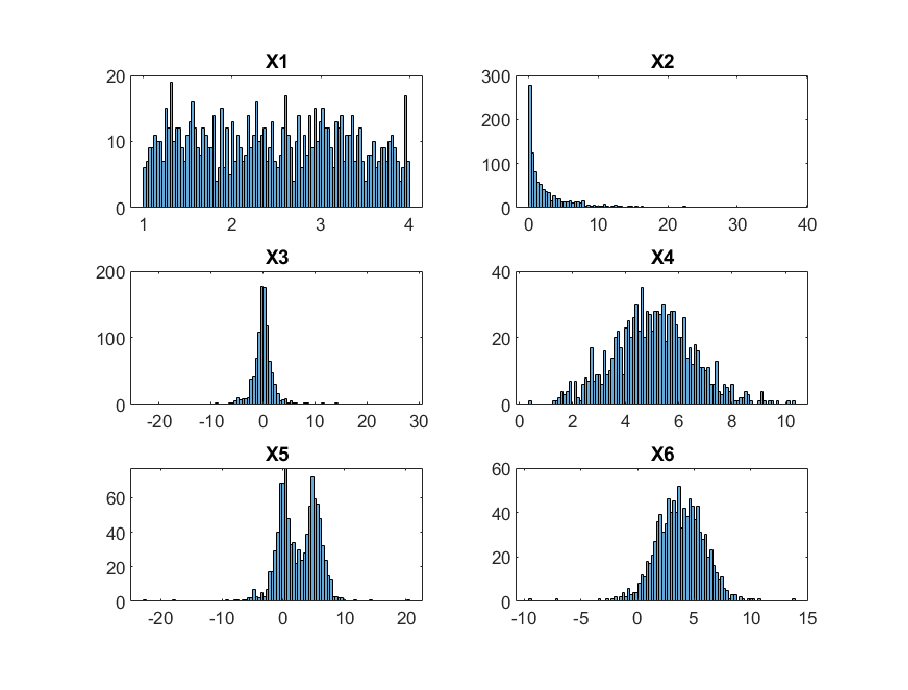
\includegraphics[width=\maxwidth{56.196688409433015em}]{figure_0.eps}
\end{center}



\vspace{1em}
\begin{par}
\begin{flushleft}
\textbf{8. Join data}
\end{flushleft}
\end{par}

\begin{par}
\begin{flushleft}
 Se generan dos funciones que tiene como parámetros el numero de filas y columnas (ver ayuda help xx). Además se generó una función que las grafica en plotxx ingresando esa matriz (ver help plotxx). 
\end{flushleft}
\end{par}

\begin{matlabcode}
mm = xx(1000,1)
\end{matlabcode}
\begin{matlaboutput}
mm = 1000x6    
    1.2481    0.6658   -0.0680    4.6068    4.6068    4.6068
    1.9836    2.3728    0.8851    4.3409    0.8851    2.6130
    1.0021    6.8063    1.3497    5.4130    5.4130    5.4129
    3.5097    0.9943   -0.9378    6.4354    6.4354    6.4353
    2.9458    6.7209    2.6543    7.1215    7.1215    7.1215
    2.4874    5.1302   -0.0041    3.8764    3.8764    3.8764
    2.2193    1.3616    1.9747    5.9487    5.9487    5.9487
    3.7295    2.5259   -0.3055    5.7366   -0.3055    2.7156
    3.6043    2.7302    1.4830    5.2308    1.4830    3.3568
    1.0670    1.6609    2.3337    5.8602    2.3337    4.0972

\end{matlaboutput}
\begin{matlabcode}
plotxx(mm, 1000, 1)
\end{matlabcode}
\begin{matlaboutput}
mm = 1000x6    
    1.8728    6.7653   -0.4424    8.2931   -0.4424    3.9250
    3.8093    3.4523    0.6370    3.4227    0.6370    2.0299
    1.0305    3.2077    7.7762    3.8435    7.7762    5.8100
    3.4648    0.4292    0.1101    4.8939    4.8939    4.8940
    3.7272    0.8016   -0.3194    7.1762   -0.3194    3.4284
    3.9502    4.5471    3.1631    4.5908    4.5908    4.5907
    1.3850    2.4667   -0.8574    4.4311    4.4311    4.4312
    2.9998    4.5163    0.4877    5.0736    5.0736    5.0737
    1.5032    4.7756   -2.1526    6.2832    6.2832    6.2831
    2.2015    0.4990    0.4090    7.7917    0.4090    4.1004

\end{matlaboutput}

\matlabheading{Parte 3. Operaciones con matrices y funciones}


\vspace{1em}
\begin{par}
\begin{flushleft}
1. Genere una matriz (mm) cuyas columnas sean cada una de las variables del problema 3, ahora tomando cada vector en R\textasciicircum{}10
\end{flushleft}
\end{par}

\begin{matlabcode}
mm = xx(10, 1)
\end{matlabcode}
\begin{matlaboutput}
mm = 10x6    
    3.3668    1.4970   -0.4948    4.9252    4.9252    4.9251
    2.7705    3.2422   -0.5291    4.5532    4.5532    4.5532
    3.5197    0.9525    0.7873    3.5893    3.5893    3.5891
    2.4636    2.1641    0.5941    6.2904    0.5941    3.4422
    1.0591    6.1624    1.8378    1.2628    1.2628    1.2627
    3.1692    4.4258   -1.7080    6.5632   -1.7080    2.4276
    3.3143    1.1920    0.1785    4.1063    4.1063    4.1065
    1.4128    4.1334    0.0476    5.4140    0.0476    2.7309
    3.0749    2.7059   -2.9046    5.6032   -2.9046    1.3493
    3.9967    3.7886    1.1095    4.3745    4.3745    4.3745

\end{matlaboutput}

\begin{par}
\begin{flushleft}
2. Genere un vector fila SUMM con la suma de las filas 2,3 y 5 de la matriz. Compruebe sus resultados.
\end{flushleft}
\end{par}

\begin{matlabcode}
summ = mm(2,:) + mm(3,:) + mm(5,:)
\end{matlabcode}
\begin{matlaboutput}
summ = 1x6    
    7.3493   10.3571    2.0960    9.4053    9.4053    9.4051

\end{matlaboutput}
\begin{matlabcode}
summ
\end{matlabcode}
\begin{matlaboutput}
summ = 1x6    
    7.3493   10.3571    2.0960    9.4053    9.4053    9.4051

\end{matlaboutput}
\begin{matlabcode}

\end{matlabcode}

\begin{par}
\begin{flushleft}
3. Genere una sentencia que cuente y ubique el número de elementos de la matriz mayores a 0.5. 
\end{flushleft}
\end{par}

\begin{matlabcode}
size(mm(mm > 0.5))
\end{matlabcode}
\begin{matlaboutput}
ans = 1x2    
    51     1

\end{matlaboutput}
\begin{matlabcode}

\end{matlabcode}

\begin{par}
\begin{flushleft}
Genere una matriz FF con los elementos de la matriz mayores a 0.5 y NAN en los otros.
\end{flushleft}
\end{par}

\begin{matlabcode}
ff_1 = mm(mm > 0.5)
\end{matlabcode}
\begin{matlaboutput}
ff_1 = 51x1    
    3.3668
    2.7705
    3.5197
    2.4636
    1.0591
    3.1692
    3.3143
    1.4128
    3.0749
    3.9967

\end{matlaboutput}
\begin{matlabcode}
ff_2 = mm(isnan(mm))
\end{matlabcode}
\begin{matlaboutput}
ff_2 =

  0x1 empty double column vector
\end{matlaboutput}

\begin{par}
\begin{flushleft}
4. Genere una matriz D con las dos primeras columnas de la matrizy una matriz DD con las dos  ultimas filas.
\end{flushleft}
\end{par}

\begin{matlabcode}
d = mm(:, 1:2)
\end{matlabcode}
\begin{matlaboutput}
d = 10x2    
    3.3668    1.4970
    2.7705    3.2422
    3.5197    0.9525
    2.4636    2.1641
    1.0591    6.1624
    3.1692    4.4258
    3.3143    1.1920
    1.4128    4.1334
    3.0749    2.7059
    3.9967    3.7886

\end{matlaboutput}


\vspace{1em}
\begin{matlabcode}
dd = mm(end-1:end, :)
\end{matlabcode}
\begin{matlaboutput}
dd = 2x6    
    3.0749    2.7059   -2.9046    5.6032   -2.9046    1.3493
    3.9967    3.7886    1.1095    4.3745    4.3745    4.3745

\end{matlaboutput}

\begin{par}
\begin{flushleft}
5. Replique la matriz dentro de una matriz mayor ZZ con el siguiente patron: e veces hacia el lado y dos veces hacia abajo.
\end{flushleft}
\end{par}

\begin{matlabcode}
%%zz = mm(y,e)
\end{matlabcode}

\begin{par}
\begin{flushleft}
6. Genere un vector VECT con 8 numeros equidistribuidos entre 2 y 3.
\end{flushleft}
\end{par}

\begin{matlabcode}
vect = linspace(2,3,8)
\end{matlabcode}
\begin{matlaboutput}
vect = 1x8    
    2.0000    2.1429    2.2857    2.4286    2.5714    2.7143    2.8571    3.0000

\end{matlaboutput}

\begin{par}
\begin{flushleft}
7. Calcule VECT’*VECT VECT.*VECT y VECT*VECT’. Explique las diferencias entre los resultados obtenidos.
\end{flushleft}
\end{par}

\begin{matlabcode}
result_1 = vect'*vect.*vect
\end{matlabcode}
\begin{matlaboutput}
result_1 = 8x8    
    8.0000    9.1837   10.4490   11.7959   13.2245   14.7347   16.3265   18.0000
    8.5714    9.8397   11.1953   12.6385   14.1691   15.7872   17.4927   19.2857
    9.1429   10.4956   11.9417   13.4810   15.1137   16.8397   18.6589   20.5714
    9.7143   11.1516   12.6880   14.3236   16.0583   17.8921   19.8251   21.8571
   10.2857   11.8076   13.4344   15.1662   17.0029   18.9446   20.9913   23.1429
   10.8571   12.4636   14.1808   16.0087   17.9475   19.9971   22.1574   24.4286
   11.4286   13.1195   14.9271   16.8513   18.8921   21.0496   23.3236   25.7143
   12.0000   13.7755   15.6735   17.6939   19.8367   22.1020   24.4898   27.0000

\end{matlaboutput}
\begin{matlabcode}
result_2 = vect*vect'
\end{matlabcode}
\begin{matlaboutput}
result_2 = 50.8571
\end{matlaboutput}

\begin{par}
\begin{flushleft}
La diferencia de resultados se debe a la diferencia en cálculo de matrices. Cuando en MATLAB se ocupa .* lo que se indica es que se multuplica elemento por elemento del arreglo (o matriz), entonces, cuando se hacen operaciones se mantendrá el rango y las dimensiones de este. Mientras que si se multiplica solo con * se ejecutará la multiplicación de matrices, cambiando las dimensiones de estas. En este caso como son dos matrices idénticas y cuadradas, por idempotencia su valor es el de la traza por su identidad. 
\end{flushleft}
\end{par}

\matlabheading{Parte 4. Modelo con simulación de Montecarlo}

\begin{par}
\begin{flushleft}
Supongamos ahora que cuenta con los resultados de una encuesta a 3000 habitantes cuyas respuestas se tabulan en 6 variables que simularemos en base a los vectores del ejercicio 3. Usted cree que estas variables se combinan en el modelo a continuaci ́on:
\end{flushleft}
\end{par}

\begin{par}
$$\begin{array}{l}
Y=a_1 \log \left(X_1 \right)+a_2 X_2 +a_3 X_3 +a_4 X_4 +a_5 X_5 +a_6 X_6 +\textrm{error}\\

\end{array}$$
\end{par}

\begin{par}
\begin{flushleft}
Donde  ${X_{a\;} =\;a}_1 \log \left(X_1 \right)+a_2 X_2 +a_3 X_3 +a_4 X_4 +a_5 X_5 +a_6 X_6$
\end{flushleft}
\end{par}

\begin{par}
\begin{flushleft}
1.Generaremos la matriz $X_{a\;}$como se indica arriba
\end{flushleft}
\end{par}

\begin{matlabcode}
x_ia = xx(3000,1)
\end{matlabcode}
\begin{matlaboutput}
x_ia = 3000x6    
    3.8860    0.9032    0.2203    4.5715    0.2203    2.3959
    2.4276    2.0023   -0.4749    6.6985   -0.4749    3.1118
    3.3832    2.7403   -1.5031    5.8626    5.8626    5.8625
    2.4021    3.0106   -0.6916    4.3498    4.3498    4.3498
    3.0942    3.0387   -0.2265    4.1311    4.1311    4.1309
    1.6115    1.7999   -1.2484    3.4847    3.4847    3.4847
    2.8430    0.4987    0.3949    3.9532    3.9532    3.9533
    2.8409    3.5700    0.2253    3.6003    3.6003    3.6005
    3.6314    1.9941    0.4184    3.1715    0.4184    1.7950
    1.2857    4.0213   -0.6039    4.1980    4.1980    4.1982

\end{matlaboutput}
\begin{matlabcode}
x_ia(:,1) = log(x_ia(:,1))
\end{matlabcode}
\begin{matlaboutput}
x_ia = 3000x6    
    1.3574    0.9032    0.2203    4.5715    0.2203    2.3959
    0.8869    2.0023   -0.4749    6.6985   -0.4749    3.1118
    1.2188    2.7403   -1.5031    5.8626    5.8626    5.8625
    0.8763    3.0106   -0.6916    4.3498    4.3498    4.3498
    1.1295    3.0387   -0.2265    4.1311    4.1311    4.1309
    0.4772    1.7999   -1.2484    3.4847    3.4847    3.4847
    1.0449    0.4987    0.3949    3.9532    3.9532    3.9533
    1.0441    3.5700    0.2253    3.6003    3.6003    3.6005
    1.2896    1.9941    0.4184    3.1715    0.4184    1.7950
    0.2513    4.0213   -0.6039    4.1980    4.1980    4.1982

\end{matlaboutput}
\begin{matlabcode}
x_a = x_ia(:,1) + x_ia(:,2) + x_ia(:,3) + x_ia(:,4) + x_ia(:,5) + x_ia(:,6)
\end{matlabcode}
\begin{matlaboutput}
x_a = 3000x1    
    9.6685
   11.7497
   20.0437
   16.2447
   16.3348
   11.4828
   13.7981
   15.6405
    9.0872
   16.2630

\end{matlaboutput}

\begin{par}
\begin{flushleft}
2. Suponga que Y es una variable aleatoria que se comporta como una exponencial(0.5). Genere Y utilizando rand.
\end{flushleft}
\end{par}

\begin{matlabcode}
y = exp(0.5) + rand(3000,1)
\end{matlabcode}
\begin{matlaboutput}
y = 3000x1    
    1.7713
    2.6232
    1.9259
    2.5164
    2.2555
    2.0417
    1.8183
    2.2232
    2.4283
    2.1879

\end{matlaboutput}
\begin{matlabcode}

\end{matlabcode}

\begin{par}
\begin{flushleft}
3. Encuentre el vector de parametros ai que resuelven el sistema lineal (1).
\end{flushleft}
\end{par}

\begin{matlabcode}
regress(y, x_ia)
\end{matlabcode}
\begin{matlaboutput}
ans = 6x1    
    0.6351
    0.0582
   -0.0040
   58.8780
   58.6139
 -117.2282

\end{matlaboutput}
\begin{matlabcode}

\end{matlabcode}

\begin{par}
\begin{flushleft}
4. Elabore un programa que le permita encontrar los vectores de parametros para 500 muestras (debe generarlas) de la encuesta. Debe guardar cada conjunto de parametros como una fila en una matriz BETAS500×6.
\end{flushleft}
\end{par}

\begin{matlabcode}
betas500 = fitlm(x_ia,y)
\end{matlabcode}
\begin{matlaboutput}
betas500 = 
Linear regression model:
    y ~ 1 + x1 + x2 + x3 + x4 + x5 + x6

Estimated Coefficients:
                    Estimate        SE         tStat      pValue 
                   __________    _________    ________    _______

    (Intercept)        2.1384     0.022347      95.691          0
    x1              0.0088754     0.013493     0.65776    0.51074
    x2              0.0026185    0.0020689      1.2657    0.20574
    x3             -0.0020154    0.0017342     -1.1622    0.24526
    x4                 6.6875       25.422     0.26307    0.79252
    x5                 6.6862       25.422     0.26301    0.79256
    x6                -13.376       50.843    -0.26308    0.79251


Number of observations: 3000, Error degrees of freedom: 2993
Root Mean Squared Error: 0.283
R-squared: 0.0019,  Adjusted R-Squared: -9.96e-05
F-statistic vs. constant model: 0.95, p-value = 0.458
\end{matlaboutput}
\begin{matlabcode}

\end{matlabcode}

\begin{par}
\begin{flushleft}
5. Encuentre la distribucion empırica de los regresores del modelo: la media de cada parametro y su mediana.
\end{flushleft}
\end{par}

\begin{matlabcode}
betas500.Coefficients
\end{matlabcode}
\begin{matlabtableoutput}
{
\begin{tabular} {|c|c|c|c|c|}\hline
\mlcell{ } & \mlcell{Estimate} & \mlcell{SE} & \mlcell{tStat} & \mlcell{pValue} \\ \hline
\mlcell{1 (Intercept)} & \mlcell{2.1384} & \mlcell{0.0223} & \mlcell{95.6910} & \mlcell{0} \\ \hline
\mlcell{2 x1} & \mlcell{0.0089} & \mlcell{0.0135} & \mlcell{0.6578} & \mlcell{0.5107} \\ \hline
\mlcell{3 x2} & \mlcell{0.0026} & \mlcell{0.0021} & \mlcell{1.2657} & \mlcell{0.2057} \\ \hline
\mlcell{4 x3} & \mlcell{-0.0020} & \mlcell{0.0017} & \mlcell{-1.1622} & \mlcell{0.2453} \\ \hline
\mlcell{5 x4} & \mlcell{6.6875} & \mlcell{25.4216} & \mlcell{0.2631} & \mlcell{0.7925} \\ \hline
\mlcell{6 x5} & \mlcell{6.6862} & \mlcell{25.4216} & \mlcell{0.2630} & \mlcell{0.7926} \\ \hline
\mlcell{7 x6} & \mlcell{-13.3758} & \mlcell{50.8432} & \mlcell{-0.2631} & \mlcell{0.7925} \\ 
\hline
\end{tabular}
}
\end{matlabtableoutput}
\begin{center}
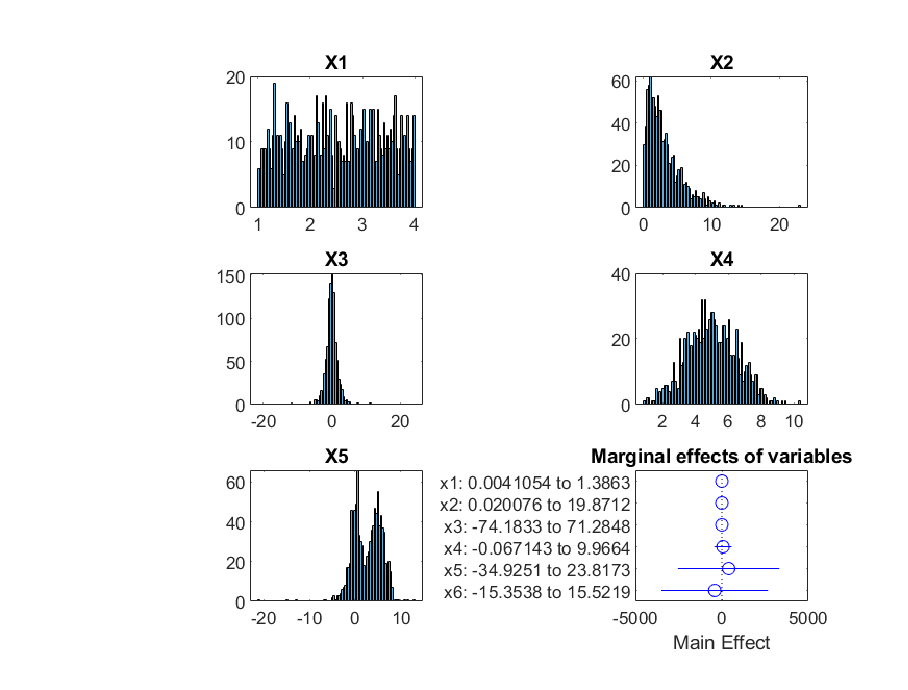
\includegraphics[width=\maxwidth{56.196688409433015em}]{figure_1.eps}
\end{center}

\begin{par}
\begin{flushleft}
6. Representación de los regresores
\end{flushleft}
\end{par}

\begin{matlabcode}
plotEffects(betas500)
title("Marginal effects of variables")
\end{matlabcode}

\matlabheading{Seguimiento MatLab}

\matlabheadingtwo{Parte 1. Distribución}

\begin{par}
\begin{flushleft}
1.Utilizando el output de la funcion de la matriz genere una matriz NN300×6. A partir de ella genere una matriz CC7×6 en la cual las primeras filas detallen la media, la desviación estándar, el mınimo, el maximo, y la mediana de cada columna de NN.
\end{flushleft}
\end{par}

\begin{matlabcode}
nn = xx(300,1)
cc = [mean(nn)' std(nn)'  min(nn)' max(nn)' median(nn)']

\end{matlabcode}

\matlabheadingtwo{2 Bucles}

\begin{par}
\begin{flushleft}
1. Genere un bucle (for) que grafique los ejercicios 3.7 y 5.6 de una forma más eficiente. 
\end{flushleft}
\end{par}

\begin{par}
\begin{flushleft}
\textbf{Para ello cree una función }\textit{\textbf{plotxx}}
\end{flushleft}
\end{par}

\begin{par}
\begin{flushleft}
2. Genere un programa que:
\end{flushleft}
\end{par}

\begin{par}
\begin{flushleft}
(a) Genere una matriz HH20×6 con la funcion del ejercicio 3.
\end{flushleft}
\end{par}

\begin{matlabcode}
hh = xx(20,1)
\end{matlabcode}

\begin{par}
\begin{flushleft}
(b) Si la suma de los elementos de la fila 1 es par, genere otra matriz. De lo contrario mantenga
\end{flushleft}
\end{par}

\begin{matlabcode}
for n = 1:length(hh)
if sum(hh(1,:)) > 2*n
    xx(20,1)
else 
    hh
end
end
\end{matlabcode}

\begin{par}
\begin{flushleft}
(c) Genere una matriz ZZ1×i cuya dimension columnas sea dinamica. En cada nuevo loop debe ir agregando un nuevo elemento al final de la fila 1.
\end{flushleft}
\end{par}

\begin{matlabcode}
for i = 1:i+1
zz = xx(1,i)
end;
\end{matlabcode}

\begin{par}
\begin{flushleft}
(d) Estos elementos se escogeran de esta forma: comenzando con la columna 1, se van tomando los elementos fila a fila, uno por loop. Si se termina la columna, comenzamos con el elemento 1 de la columna 2 etc.
\end{flushleft}
\end{par}

\begin{matlabcode}
for i = 1:i+1
zz = xx(1,i)
select = zz(1,i)
end;
\end{matlabcode}

\begin{par}
\begin{flushleft}
(e) El proceso de generaci on de la matriz HH debe detenerse cuando la suma de sus elementos alcance el valor 50. Ayuda: busque la funci ́on while.
\end{flushleft}
\end{par}

\begin{matlabcode}
while sum(hh, "all") == 50
for n = 1:length(hh)
if sum(hh(1,:)) > 2*n
    xx(20,1)
else 
    hh
end
end;
\end{matlabcode}

\begin{par}
\begin{flushleft}
(f) Finalmente, encuentre y señale la posicion del  ultimo elemento agregado en la matriz original HH utilizando una sentencia del tipo “El elemento nrox de la matriz ZZ se encuentra en la posicion r, c en la matriz HH”. Ayuda: busque la funcion disp.
\end{flushleft}
\end{par}

\begin{matlabcode}
while sum(zz, "all") == 50
for i = 1:i+1
zz = xx(1,i)
end
out=double(extract(string(zz),2))';
disp(out)
\end{matlabcode}

\end{document}
